\documentclass[11pt,aspectratio=169]{beamer}
 
\usetheme[sectionpage=none, subsectionpage=none, progressbar=none]{metropolis}           % Use metropolis theme
 
  \usepackage{outlines}
  \usepackage{caption}
  \usepackage{appendixnumberbeamer}
  \usepackage{booktabs}
  \usepackage{tcolorbox}
  \usepackage{tabularx}
  \usepackage[export]{adjustbox}[2011/08/13]
  \usepackage{bm}
  
  \def\shrug{\texttt{\raisebox{0.75em}{\char`\_}\char`\\\char`\_\kern-0.5ex(\kern-0.25ex\raisebox{0.25ex}{\rotatebox{45}{\raisebox{-.75ex}"\kern-1.5ex\rotatebox{-90})}}\kern-0.5ex)\kern-0.5ex\char`\_/\raisebox{0.75em}{\char`\_}}}


\newcolumntype{R}{>{\raggedleft\arraybackslash}X} 

\newtheorem*{defn}{Def'n}

\DeclareUnicodeCharacter{2212}{-}

  
 \setbeamertemplate{footline}[frame number]{}

\setbeamertemplate{footline}{% 
  \hfill% 
  \usebeamercolor[fg]{page number in head/foot}% 
  \usebeamerfont{page number in head/foot}% 
  \insertframenumber%
  %\,/\,\inserttotalframenumber
  \kern1em\vskip2pt% 
}

\makeatletter
\setbeamertemplate{headline}{%
  \begin{beamercolorbox}[colsep=1.5pt]{upper separation line head}
  \end{beamercolorbox}
  \begin{beamercolorbox}{section in head/foot}
    \vskip2pt\insertnavigation{\paperwidth}\vskip2pt
  \end{beamercolorbox}%
  \begin{beamercolorbox}[colsep=1.5pt]{lower separation line head}
  \end{beamercolorbox}
}
\let\@@magyar@captionfix\relax % IMPORTANT: This is a workaround to fix a random eror with the 2018 installation
\makeatother

\usepackage{xcolor} 
\listfiles

\setbeamercolor{section in head/foot}{fg=normal text.bg, bg=structure.fg}

    \usepackage{smartdiagram}
    \usepackage{tikz}
\usetikzlibrary{shapes.geometric, arrows}
\tikzstyle{startstop} = [rectangle, rounded corners, minimum width=3cm, minimum height=1cm,text centered, draw=black, fill=red!30]
\tikzstyle{io} = [trapezium, trapezium left angle=70, trapezium right angle=110, minimum width=3cm, minimum height=1cm, text centered, draw=black, fill=blue!30]
\tikzstyle{process} = [rectangle, minimum width=3cm, minimum height=1cm, text centered, draw=black, fill=orange!30]
\tikzstyle{decision} = [diamond, minimum width=3cm, minimum height=1cm, text centered, draw=black, fill=green!30]

\title{Gov 2006: Formal Political Theory II \\
Section 9}
\date{\today}
\author{ \textbf{Sophie Hill}}


\begin{document}
  \maketitle
  
 %%%%%%%%%%%%%%%%%%%%%%%%%%%%%%%%%%%%%%%%%%
\begin{frame}{Today}

\Large

\begin{itemize}
\setlength{\itemsep}{1em}
\item PSET practice 
\begin{itemize}
\large
\item The basic legislative bargaining model from Baron \& Ferejohn
\item Finishing up part (d) from PSET 6 Q4!
\end{itemize}
\item Multiparty spatial modelling 
\begin{itemize}
\large
\item Theory: Cox (1990)
\item Empirics: Ezrow (2008); Tsebelis \& Crosson (2017)
\end{itemize}
\end{itemize}

\end{frame}
%%%%%%%%%%%%%%%%%%%%%%%%%%%%%%%%%%%%%%%%%%
\begin{frame}{Legislative bargaining}

Next week we will read Baron \& Ferejohn (1989), a seminal paper on \alert{legislative bargaining}.

\vspace{1em}

A version of this model may (?) end up on the next problem set, so let's go through a simple practice problem today!

\end{frame}
%%%%%%%%%%%%%%%%%%%%%%%%%%%%%%%%%%%%%%%%%%
\begin{frame}{Legislative bargaining}

\textbf{Set-up:}

\begin{itemize}
\item Legislature with $n$ members, who divide rents $r$ (normalized to 1) among themselves
\item They only care about rents: $w^i(r) = r$
\item Discount rate = $\delta \in [0,1]$
\end{itemize}

\pause 

\textbf{Timing:}

\begin{enumerate}
\item A member has proposed an allocation of $r$.
\item Legislature votes $\{yay, nay\}$ on the proposed allocation under simple majority rule.
\item If the proposition is not passed, then a new member is randomly chosen (with $p = \frac{1}{n}$) to propose an allocation of $r$.
\item This proposal is voted on, and if it does not pass, then all rents are dissipated.
\end{enumerate}

\end{frame}
%%%%%%%%%%%%%%%%%%%%%%%%%%%%%%%%%%%%%%%%%%
\begin{frame}{Legislative bargaining}

\textbf{Question 1(a)}: What is the allocation proposed in the first period?

\textbf{Solution}: Solve by backwards induction. What allocation would be chosen in the 2nd proposal? 
\pause 
\begin{itemize}
\item Given that all rents are dissipated if the 2nd proposal is rejected, the member will choose to allocate all of $r$ to herself. 
\item Legislature accepts, since they get zero rents either way. 
\end{itemize} 
\pause

What is the continuation value of the game in the first stage?

\begin{tcolorbox}
\textbf{Def'n}: The \textit{continuation value} is the present value of the equilibrium payoff stream for a given player.
\end{tcolorbox}

\end{frame}

%%%%%%%%%%%%%%%%%%%%%%%%%%%%%%%%%%%%%%%%%%
\begin{frame}{Legislative bargaining}

\textbf{Solution (cont'd)}: The continuation value for a given member is the probability of being chosen in the 2nd stage $\times$ the discounted value of the equilibrium rents:

$$ V = \frac{1}{n} \cdot \delta \cdot 1 = \frac{\delta}{n}$$

So, what does the stage 1 proposer $p_1$ choose? \pause Need to offer at least the continuation value to a minimal winning coalition $\mathcal{C}$, such that $|\mathcal{C}| = \frac{n-1}{2}$. (\alert{Why?}) \pause 

\[
a_i^* = 
\begin{cases}
1 - \frac{\delta}{n} \left( \frac{n-1}{2} \right) & \text{if } i = p_1 \\
\frac{\delta}{n} & \text{for } \frac{n-1}{2} \text{ randomly-chosen members } \in \mathcal{N}\setminus{\{p_1\}} \\
0 & \text{for } \frac{n-1}{2} \text{ randomly-chosen members } \in \mathcal{N}\setminus{\{p_1\}}  \\

\end{cases}
\]


\end{frame}
%%%%%%%%%%%%%%%%%%%%%%%%%%%%%%%%%%%%%%%%%%
\begin{frame}{Legislative bargaining}

\textbf{Question 1(b)}: How does the advantage of the first proposer vary with the size of the legislature? \pause

\textbf{Solution}: Compare the expected payoffs of the proposer vs other members. \pause 
\begin{itemize}
\item The agenda-setter keeps $1 - \frac{\delta}{n} \left( \frac{n-1}{2} \right)$ for herself. \pause 
\item What is the expected payoff for the other members? \pause $\frac{\delta}{2n}$ \pause 
\item Both expected payoffs are decreasing in $n$ \pause 
\item What about the difference (i.e. the advantage of the agenda-setter)? \pause It has range $ \lbrack 1 - \frac{\delta}{3}, 1 - \frac{\delta}{2} \rbrack $, at its maximum when $n=3$ and decreasing as $n \rightarrow \infty$.

\end{itemize}


\end{frame}
%%%%%%%%%%%%%%%%%%%%%%%%%%%%%%%%%%%%%%%%%%
\begin{frame}{Legislative bargaining}

\textbf{Question 1(c)}: Now suppose that the stage game in which a member is randomly chosen to propose an allocation is repeatedly \alert{infinitely many times}. Show that the allocation in (a) is also an equilibrium of the infinitely repeated game. \pause 

\textbf{Solution}: We solve using backward induction: 

\begin{itemize}
\item Let the continuation value for member $i$ be $V_i$ \pause
\item Member $i$ will support any proposal giving her at least $\delta V_i$ \pause 
\item So the proposer offers $\delta V_i$ to her winning coalition, 0 to everyone else, and keeps $1 - \frac{n-1}{2} \delta V_i$ for herself
\end{itemize}


\end{frame}

%%%%%%%%%%%%%%%%%%%%%%%%%%%%%%%%%%%%%%%%%%
\begin{frame}{Legislative bargaining}

The continution value is thus the weighted combination:

\begin{align*}
 V_i &= \frac{1}{n} \left[ 1 - \frac{n-1}{2} \delta V_i \right] + \left( \frac{n-1}{2n} \right) \delta V_i \\  
 &= \frac{1}{n}
 \end{align*}
 
 \pause 
So the proposer offers $\delta V_i = \frac{\delta}{n}$ to members of the minimum winning coalition, 0 to the others, and keeps the rest for herself. This is identical to the equilibrium allocation found in part (a). 



\end{frame}

%%%%%%%%%%%%%%%%%%%%%%%%%%%%%%%%%%%%%%%%%%
\begin{frame}{Multiparty spatial modelling: motivation}

\begin{figure}
\centering
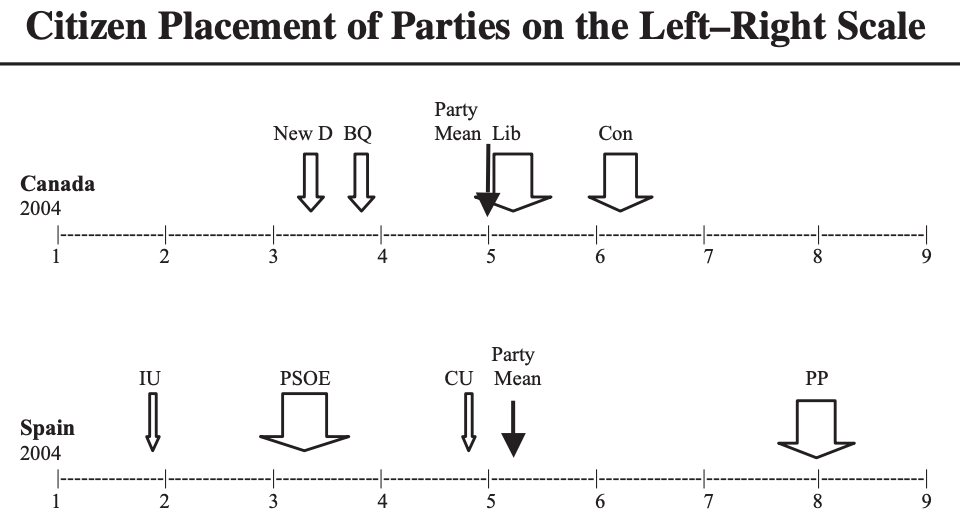
\includegraphics[width=0.75\textwidth]{dalton.png}
\caption{From Dalton (2008), ``The quantity and the quality of party systems: Party system polarization, its measurement, and its consequences.'' \textit{Comparative Political Studies}}
\end{figure}

\end{frame}
%%%%%%%%%%%%%%%%%%%%%%%%%%%%%%%%%%%%%%%%%%
\begin{frame}{Multiparty spatial modelling: motivation}



\begin{table}[]
\begin{tabular}{@{}lllll@{}}
\toprule
                                  & \textbf{Canada}         & \textbf{Spain}              &  &  \\ \midrule
\textbf{Number of parties}        & 5                       & 5                           &  &  \\
\textbf{Party polarization index} & 2.06                    & 4.33                        &  &  \\ \bottomrule
\end{tabular}
\end{table}

\end{frame}
%%%%%%%%%%%%%%%%%%%%%%%%%%%%%%%%%%%%%%%%%%
\begin{frame}{Multiparty spatial modelling: motivation}



\begin{table}[]
\begin{tabular}{@{}lllll@{}}
\toprule
                                  & \textbf{Canada}         & \textbf{Spain}              &  &  \\ \midrule
\textbf{Number of parties}        & 5                       & 5                           &  &  \\
\textbf{Party polarization index} & 2.06                    & 4.33                        &  &  \\
\textbf{Electoral system}         & Single member plurality & Proportional representation &  &  \\
\textbf{Votes per voter}         & 1 & 1 &  &  \\
\textbf{Partial abstention} & N/A & N/A & & \\
\textbf{District magnitude} & 1 & 1-35 (median=5) & & \\
 \bottomrule
\end{tabular}
\end{table}

\end{frame}
%%%%%%%%%%%%%%%%%%%%%%%%%%%%%%%%%%%%%%%%%%
\begin{frame}{Multiparty spatial modelling: Cox (1990)}

Cox (1990) identifies \alert{three} key factors that produce \textit{centripetal} incentives (central clustering), at least in non-cumulative systems. 

\begin{tcolorbox}
What are they? 
\end{tcolorbox}

\pause 
\begin{itemize}
\item number of votes per voter
\item partial abstention
\item district magnitude
\end{itemize}

\end{frame}
%%%%%%%%%%%%%%%%%%%%%%%%%%%%%%%%%%%%%%%%%%
\begin{frame}{Multiparty spatial modelling: Cox (1990)}

Cox (1990) identifies \alert{three} key factors that produce \textit{centripetal} incentives (central clustering), at least in non-cumulative systems. 

\begin{tcolorbox}
What effect do they have?
\end{tcolorbox}

Centripetal incentives are produced when:
\pause 
\begin{itemize}
\item number of votes per voter is $\{ high, low \}$
\item partial abstention $\{ permitted, not \, permitted \}$
\item district magnitude $\{ high, low \}$
\end{itemize}

\end{frame}
%%%%%%%%%%%%%%%%%%%%%%%%%%%%%%%%%%%%%%%%%%
\begin{frame}{Multiparty spatial modelling: Cox (1990)}

Cox (1990) identifies \alert{three} key factors that produce \textit{centripetal} incentives (central clustering), at least in non-cumulative systems. 

\begin{tcolorbox}
What effect do they have?
\end{tcolorbox}

Centripetal incentives are produced when:
\pause 
\begin{itemize}
\item number of votes per voter is \alert{high}
\item partial abstention \alert{ not permitted}
\item district magnitude \alert{low}
\end{itemize}

\end{frame}



%%%%%%%%%%%%%%%%%%%%%%%%%%%%%%%%%%%%%%%%%%
\begin{frame}{Multiparty spatial modelling: empirical tests}

\begin{figure}
\centering
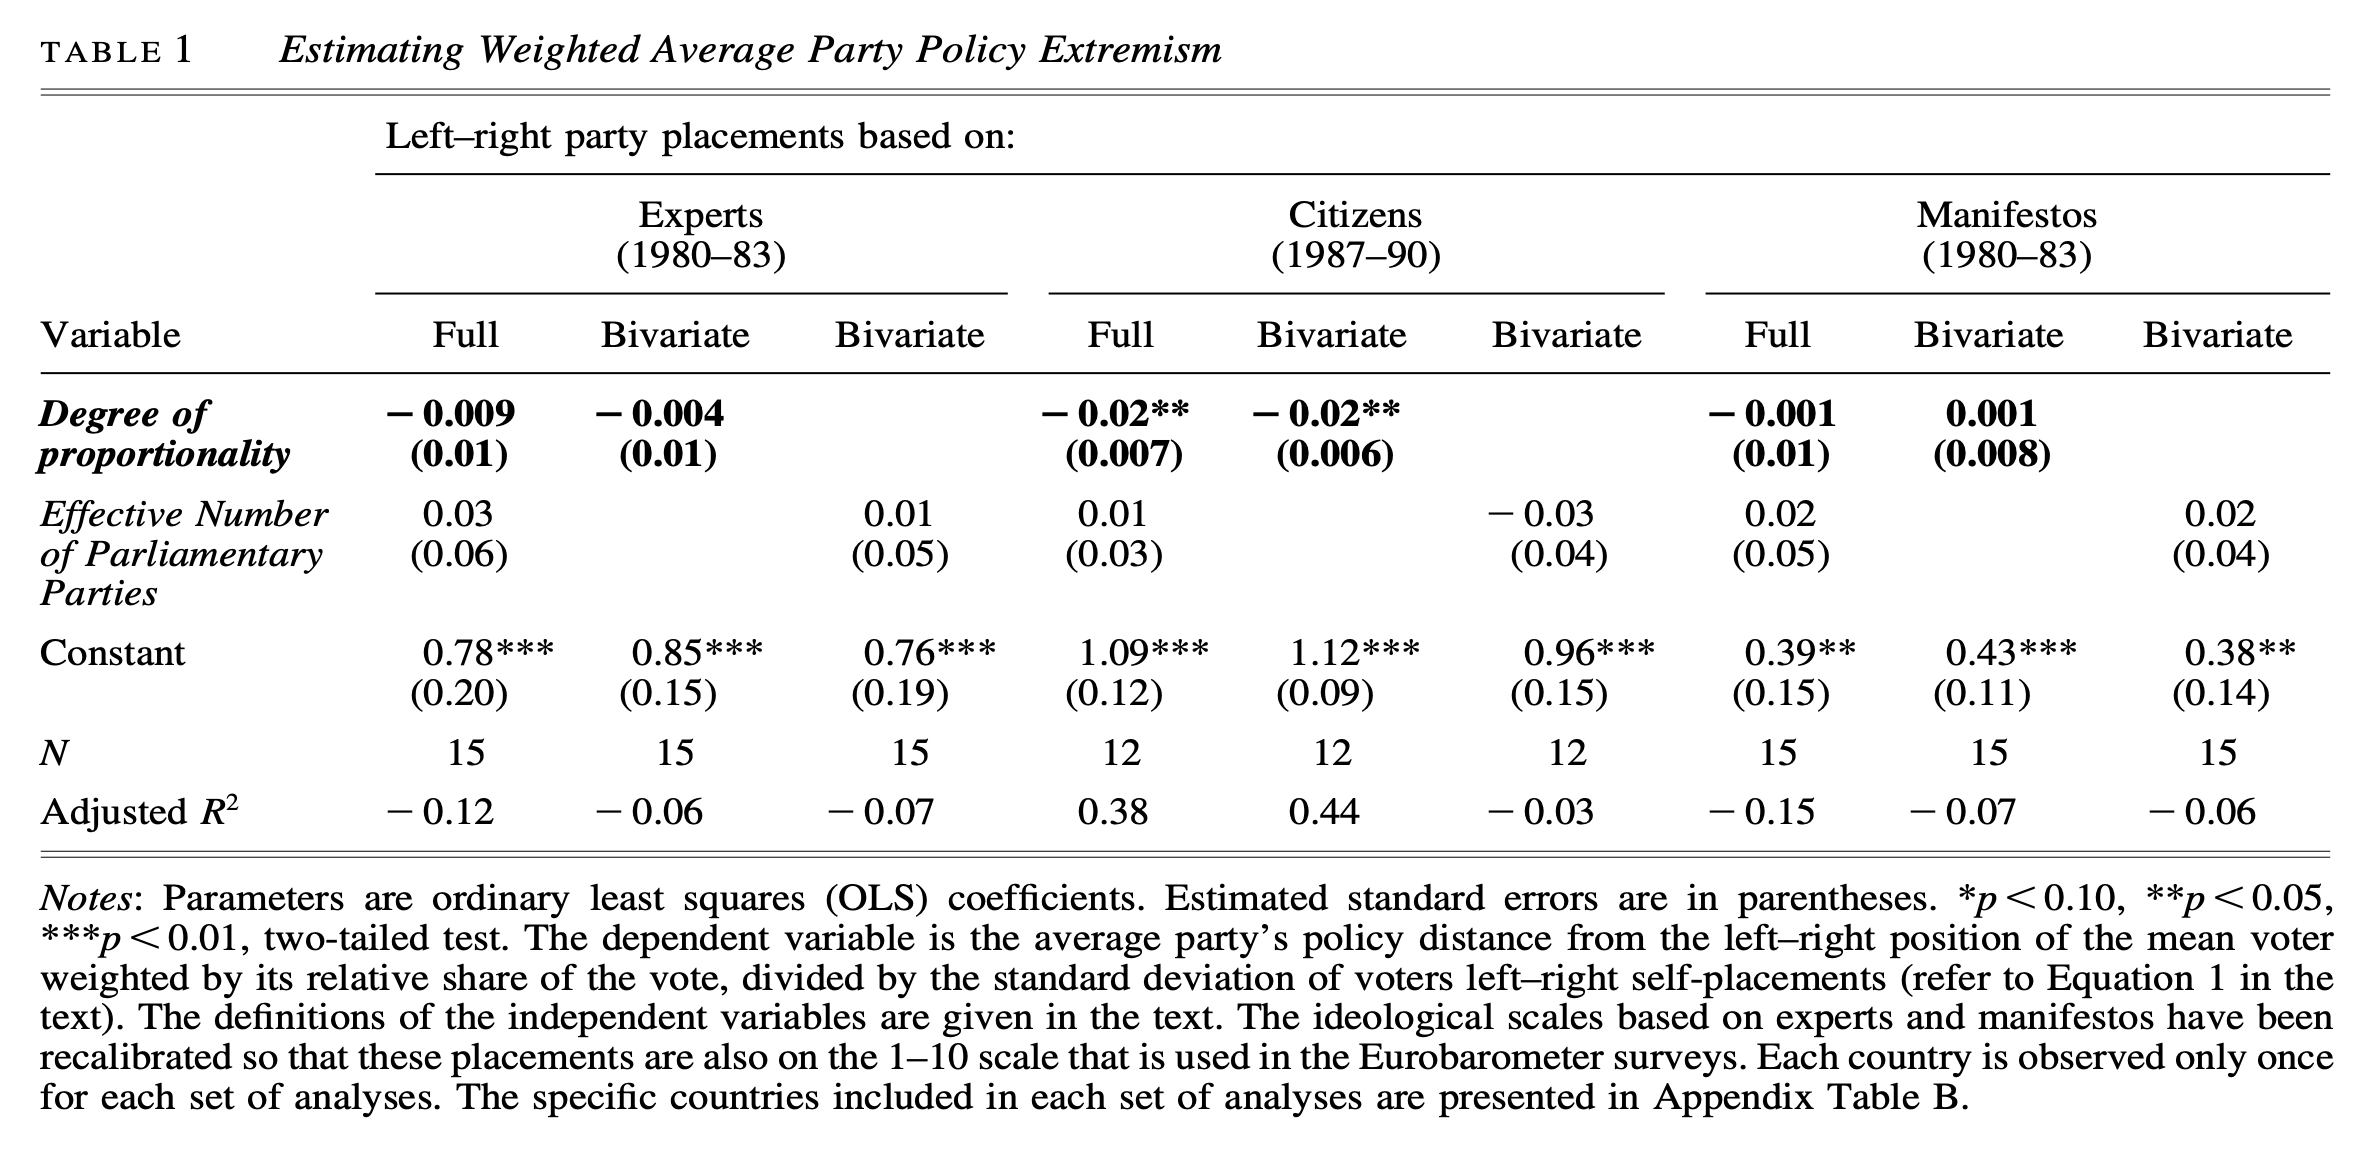
\includegraphics[width=0.8\textwidth]{reg.png}
\caption{From Ezrow (2008). ``Parties' policy programmes and the dog that didn't bark: No evidence that proportional systems promote extreme party positioning." British Journal of Political Science 38.3 (2008): 479-497.}
\end{figure}

\end{frame}
%%%%%%%%%%%%%%%%%%%%%%%%%%%%%%%%%%%%%%%%%%
\begin{frame}{Multiparty spatial modelling: empirical tests}

``The conventional understanding developed in the influential spatial modelling study by Cox is that proportional electoral rules exert centrifugal incentives that motivate parties to present non-centrist policy programmes.'' (Ezrow, 2008)

\pause 
\vspace{2em}

\begin{tcolorbox}
Is the ``conventional understanding'' correct?
\end{tcolorbox}

\end{frame}
%%%%%%%%%%%%%%%%%%%%%%%%%%%%%%%%%%%%%%%%%%
\begin{frame}{Multiparty spatial modelling: empirical tests}

\begin{figure}
\centering
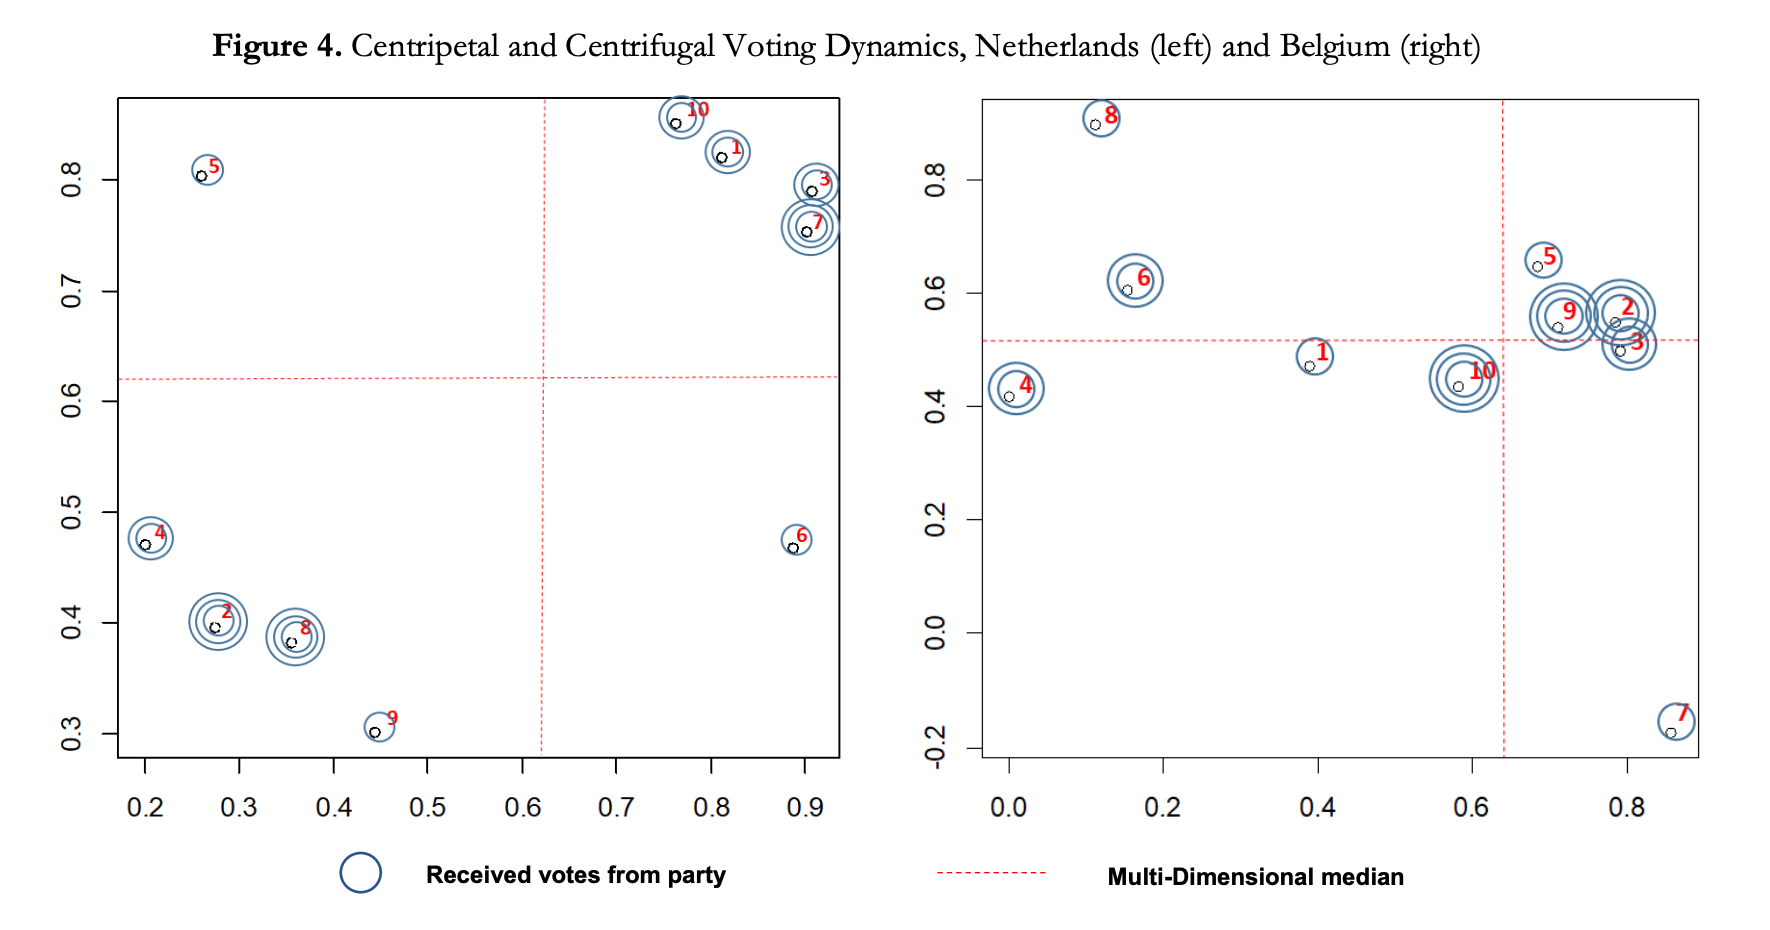
\includegraphics[width=0.8\textwidth]{crosson.png}
\caption{From Tsebelis \& Crosson (2017). ``MULTIPLE VOTE SYSTEMS: Toxin or Tonic for Political Polarization?''}
\end{figure}

\end{frame}




\end{document}
